\section{Hybrid System} % (fold)
\label{sec:hybrid_system}
As mentioned in the previous chapter, both the memory-based and disk-based
implementations of our consistent cache fail to account for data persistence.
We mentioned briefly that the most simple persistence method directly utilizes
S3 to store cached data. We believe, however, that there is more benefit than
just persistence. For the purposes of cost effectiveness, we posit that it is
useful to create a hybrid cache.

While in other versions, the cache grows incrementally without eviction,in this
variation we use only \emph{one} EC2 node and evict records into S3. We believe
that this configuration offers an effective means of storing the same quantity
of keys, with only the slight performance cost of having to query S3. The key
search function initially queries the EC2 node and upon a miss, searches in S3.

% section hybrid_system (end)

\section{Implementation} % (fold)
\label{sec:Implementation}
Within the new hybrid system, each cache node must be properly configured with
the credentials required for access to S3. Each node is then loaded with a
broker that acts as a thin interface layer between S3 and the individual node.
It is possible for each node's broker to be configured independently with a
different set of credentials or to utilize different buckets within S3 just as
it is possible for each of them to share a common set of credentials and
storage buckets. In the case of the former, persistence is only maintained for
as long as a node's S3 broker is capable of utilizing a specific bucket.

\subsection{Implementation Redesign} % (fold)
\label{sec:hybrid_redesign}
Due to previous works\cite{chiu_ccgrid11,chiu_ijngc11}, our hybrid cache system
was initially implemented in Java. During initial testing, however, we
identified a number of implementation issues that prompted a total redesign. In
order to do so and because of the implementer's greater familiarity with the
language, the redesign was done in Ruby and experiments run on MRI Ruby
1.9.2p180. Although a redesign became necessary, the implementation still
follows that which is outlined in Chapter~\ref{chap:Background}.

% subsection hybrid_redesign (end)

\subsection{Insert} % (fold)
\label{sub:hybrid_insert}
As mentioned, the hybrid cache now evicts records from its main-memory storage.
To accomodate this we now must take into account some method of eviction. For
now we will consider only the most simple case of a First-In First-Out (FIFO)
queue. Further eviction methods will be covered in
Chapter~\ref{chap:Eviction_Strategies}.

The algorithm for insertion is made more complex by the inclusion of this new
storage medium. While previously the server needed only worry about inserting
into the indexing scheme, we now need to keep an additional queue for the
purposes of eviction. Further, we must track the ``fullness'' of our indexing
scheme so that we may evict into S3 as we near our thresholds.
Algorithms~\ref{alg:hybrid_insert}-\ref{alg:hybrid_evict} detail this process.
For the sake of simplicty, we refer to the indexing scheme under the variable
$memory$ as this algorithm operates independently of its details.

\begin{algorithm}[htp]
\small
\caption{\label{alg:hybrid_insert}hybrid\_insert(key, value)}
\begin{algorithmic}[1]
\STATE $\triangleright$ Obtain the global eviction queue $memory\_queue$
\STATE $size \leftarrow value$.size

\IF{!$memory$.fits(size)}
  \STATE hybrid\_evict\_from\_memory(size)
\ENDIF

\STATE $memory$.insert(key, value)
\STATE $memory\_queue$.add(key)
\end{algorithmic}
\end{algorithm}

\begin{algorithm}[htp]
\small
\caption{\label{alg:hybrid_evict}hybrid\_evict\_from\_memory(size)}
\begin{algorithmic}[1]
\STATE $\triangleright$ Obtain the global eviction queue $memory\_queue$,
$threshold$, and $S3$ broker
\STATE $memory\_limit \leftarrow memory$.size $* threshold$

\STATE $\triangleright$ Continue evicting until our memory is beneath our
threshold and we can fit the new element in
\WHILE{$(memory\_limit > memory$.size$)$ and \@!$memory$.fits(size)}
  \STATE $\triangleright$ obtain the evicted key from our eviction queue
  \STATE $key \leftarrow memory\_queue$.shift
  \STATE $value \leftarrow memory$.search(key)
  \STATE $memory$.delete(key)
  \STATE $S3$.insert($key$, $value$)
\ENDWHILE
\end{algorithmic}
\end{algorithm}

Algorithm~\ref{alg:hybrid_insert} operates in tandom with
Algorithm~\ref{alg:hybrid_evict} to determine if the cache node's memory
contains enough free space to add the newly inserted element and, if not, evict
data into S3 until it has either dropped under our required threshold or
contains enough space to store our newly inserted element.

Insertion begins by ascertaining the size of the data being inserted into the
cache. The cache then queries whether or not there is enough space in memory to
contain the new object. If not, it triggers an eviction and we jump to
Algorithm~\ref{alg:hybrid_evict}.

Eviction is processed by looping through the eviction queue. We begin by
identifying the new required size computed from the current size of memory and
a user-specified threshold. We then loop over lines 5 through 9, retrieving the
key to be evicted and a reference to its associated data. That data is then
removed from the indexing structure before being sent to S3. We continue
looping until the size of data remaining in memory is below our required
threshold. For convenience this algorithm is presented in serial form, however
creating a parallelized version is as simple as calling eviction in a separate
thread and maintaining locks over both the eviction queue and the indexing
structure.

% subsection hybrid_insert (end)

% section Implementation (end)


\section{Hybrid Cache Evaluation} % (fold)
\label{sub:hybrid_system_evaluation}
We built the hybrid cache mentioned in Section~\ref{sec:hybrid_system} and ran
the following experiments on one {\tt m1.xlarge} node. Using 5 MB unit size, we
randomly submitted 3000 unique keys over 5000 requests. We also submitted 1000
requests over 500 unique keys for 25 MB unit size. We measured their miss
rates, as shown in Figures~\ref{fig:5mb-S3evict} and~\ref{fig:25mb-S3evict}
respectively. The subgraphs within each figure show the number of records that
have been evicted into S3. As can be seen in both figures, the hybrid cache
offers lower miss rates, which results in lower average request times. This
pattern is more prominent and occurs sooner in Figure~\ref{fig:25mb-S3evict}
due to a lower key range being used in the experiment. We do not offer the
same, in-depth cost analysis as in section~\ref{sub:performance_cost_analysis}.

\begin{figure}[htp]
\begin{center}
	\subfigure[Data Size = 5 MB]
	{\label{fig:5mb-S3evict}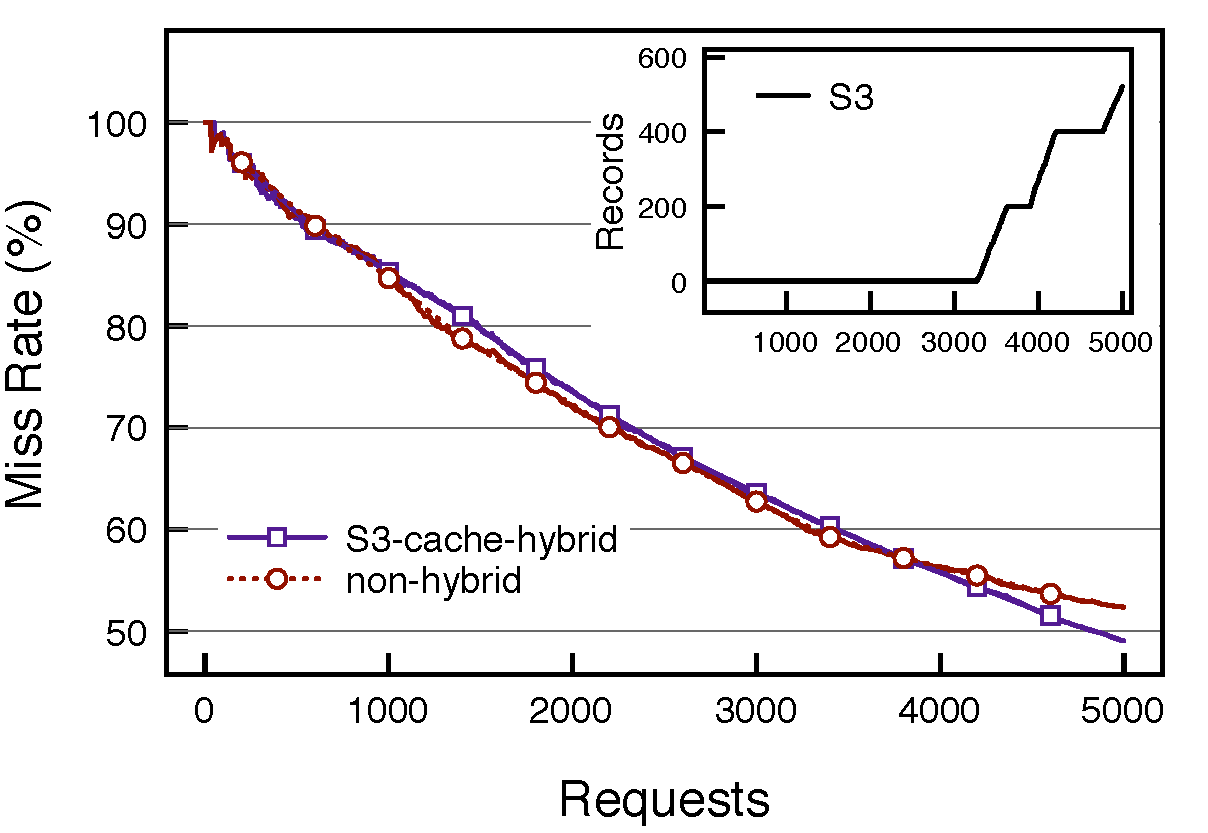
\includegraphics[scale=0.35]{figures/s3evict-05.pdf}}
	\subfigure[Data Size = 25 MB]
	{\label{fig:25mb-S3evict}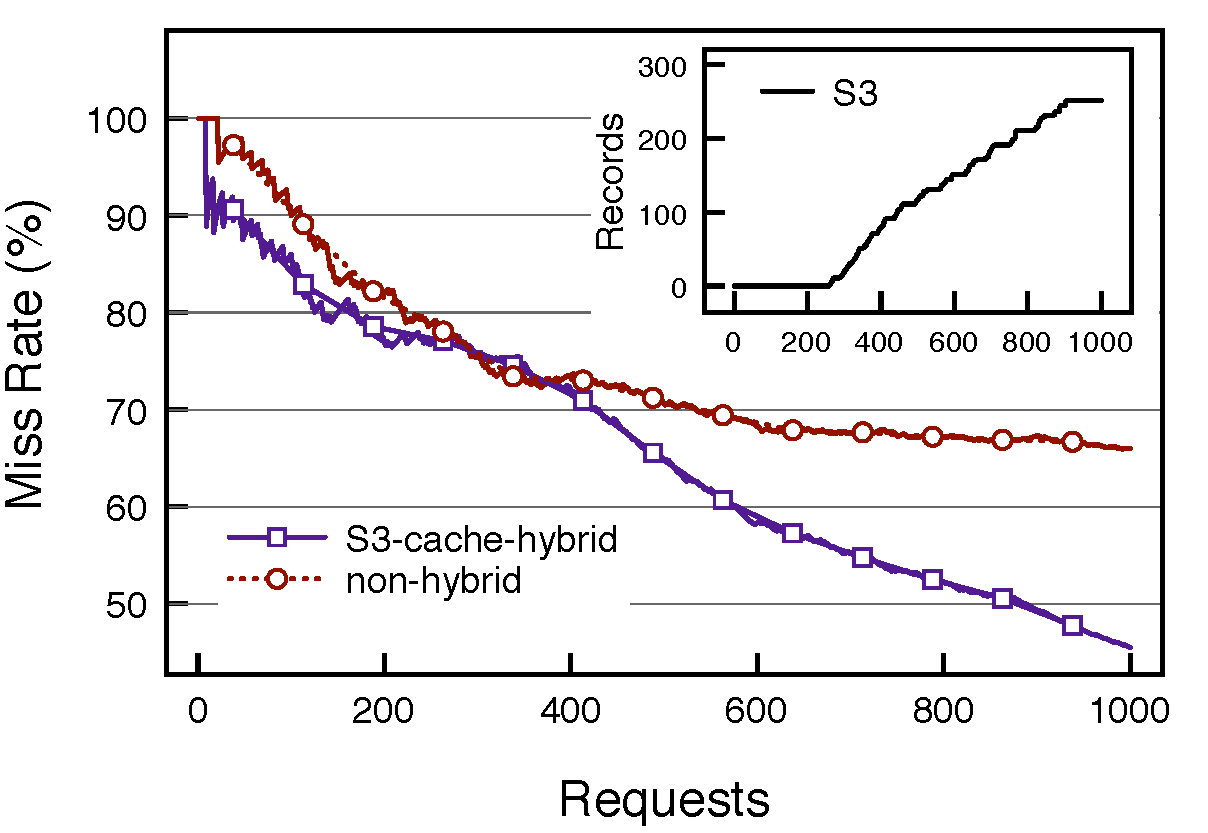
\includegraphics[scale=0.35]{figures/s3evict-25.pdf}}
	\caption{Miss Rates for S3-Eviction Hybrid Cache}
\end{center}
\end{figure}

% subsection hybrid_system_evaluation (end)
